\documentclass[a4paper, 10pt]{article}
\usepackage[english]{babel}
\usepackage[utf8]{inputenc} 
\usepackage{ragged2e}
\usepackage{tikz}
\usetikzlibrary{arrows}
\usetikzlibrary{automata, positioning}
\usepackage{lipsum}
\usepackage{enumitem}
\usepackage{pgf}
\usepackage{tikz}
\usepackage[utf8]{inputenc}
\usetikzlibrary{arrows,automata}
\usetikzlibrary{positioning}


\newcommand\blfootnote[1]{%
  \begingroup
  \renewcommand\thefootnote{}\footnote{#1}%
  \addtocounter{footnote}{-1}%
  \endgroup
}

\title{Etapa 2: Análisis Sintáctico}
\date{Enero - Marzo 2016}
\author{Benjamin Amos, Douglas Torres}

\begin{document}
	
	\maketitle
	\pagenumbering{gobble}
	\newpage
	\pagenumbering{arabic}
	
	\section{Detalles de Implementacion}
		
		\par	
		\medskip	
		Para la implementación de la segunda etapa del proyecto, utilizamos
		una herramienta, parte de la librería ply, llamada \textit{yacc}, la cual
		permite el diseño de una gramática para la creación del parser para nuestra
		lista de tokens, lo cual permitirá el diseño del árbol sintáctico abstracto, como
		finalidad de esta etapa.
		
		\par
		\medskip
		La implementacion del parser fue dividida en dos partes, un archivo para la creación
		de la gramatica libre de contexto la cual estudiara la sintaxis de un programa
		escrito en el lenguaje de estudio \textbf{BOT} y generara todas las cadenas posibles
		permitidas por el mismo, y otro archivo en el cual se almacenan las estructuras de datos
		utilizadas para la creación del árbol sintáctico abstracto, al igual que los métodos que permiten
		proporcionar la interfaz pedida.
		
		\subsection{parser.py}
		
			\par
			\medskip
			En este archivo se encuentran las reglas gramaticales permitidas por el lenguaje \textbf{BOT}.
			De este modo, se pueden producir las distintas cadenas que acepta el mismo lenguaje. Así mismo, 
			en las reglas, se encuentra la inicialización y agregación de nodos al árbol sintáctico abstracto.
			
		\subsection{arboles.py}
		
			\par
			\medskip
			Este archivo contiene las estructuras de datos utilizadas para la creación del árbol sintáctico 
			abstracto, las cuales se mencionan a continuación:
			
			\begin{enumerate}
				\item \textbf{ArbolInstr}:
				\begin{itemize}
					\item \textit{CondicionalIf}
					\item \textit{IteracionIndef}
					\item \textit{Activate}
					\item \textit{Deactivate}
					\item \textit{Advance}					
				\end{itemize}							
				\item \textbf{ArbolBin}
				\item \textbf{ArbolUn}
				\item \textbf{Ident}
				\item \textbf{Bool}
				\item \textbf{Numero}\\
			\end{enumerate}
			
			Notemos que solo se encuentran creadas estructuras de datos para el manejo de instrucciones de
			controlador de \textbf{BOT}.
	
	\newpage			
	\section{Sección Teórico-Práctica}
		
		\par
		\medskip
		En esta sección se presenta el desarrollo y respuestas para las preguntas propuestas para esta 
		etapa.
		
		\bigskip
		\begin{enumerate}[leftmargin=*]
			\item Basados en las gramáticas $G1_i$ y $G1_d$ dadas:\\
			\begin{enumerate}[label=(\alph*)]
				\item Para construir el analizador sintáctico \textit{LR(0)} de \textbf{$G1_i$}, modificamos la gramática y queda:\\
					\begin{enumerate}[label=(\roman*)]
						\item \textit{S$'$} $\rightarrow$ \textit{S}\$\\
						\item \textit{S} $\rightarrow$ \textit{Sa}\\
						\item $\hphantom{\quad}\hspace{5pt}|$ $\lambda$\\  
					\end{enumerate}

					Vemos que ocurre un conflicto \textbf{shift-reduce} en el estado $I_0$, como se ve en los siguientes estados:\\
							
					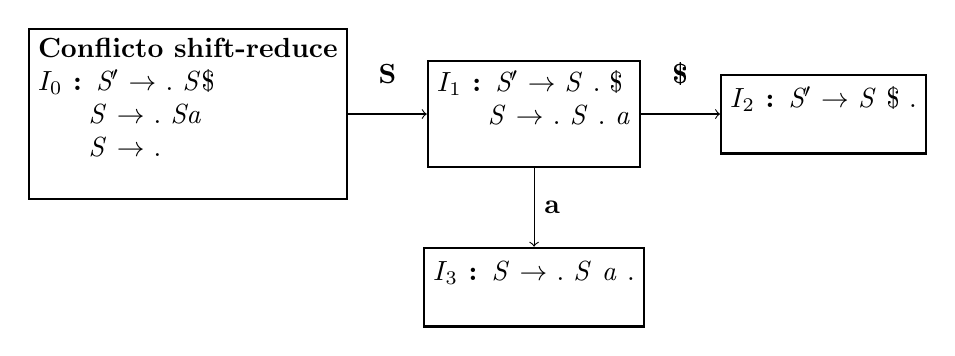
\begin{tikzpicture}[every node/.style={minimum height={1cm},thick,align=left}]
					
					\node[draw] (I0) {
						\textbf{Conflicto shift-reduce}\\
						\textbf{$I_0$ : }\textit{S$'$} $\rightarrow$ \textbf{$.$} \textit{S}\$\\
					   	$\hphantom{\quad}\hspace{5pt}$ \textit{S} $\rightarrow$ \textbf{$.$} \textit{Sa}\\
						$\hphantom{\quad}\hspace{5pt}$ \textit{S} $\rightarrow$ \textbf{$.$}\\
					};
					\node[draw, right= of I0] (I1) {
						\textbf{$I_1$ : }\textit{S$'$} $\rightarrow$ \textit{S} \textbf{$.$} \$\\
			   			$\hphantom{\quad}\hspace{5pt}$ \textit{S} $\rightarrow$ \textbf{$.$} \textit{S} \textbf{$.$} \textit{a}\\
					};
					\node[draw, right=of I1] (I2) {
						\textbf{$I_2$ : }\textit{S$'$} $\rightarrow$ \textit{S} \$ \textbf{$.$}\\
					};
					\node[draw, below=of I1] (I3) {
						\textbf{$I_3$ : }\textit{S} $\rightarrow$ \textbf{$.$} \textit{S} \textit{a} \textbf{$.$}\\
					};

					\draw[->] (I0) -- (I1) node[midway,above] {\textbf{S}};
					\draw[->] (I1) -- (I2) node[midway,above] {\textbf{\$}};
					\draw[->] (I1) -- (I3) node[midway,right] {\textbf{a}};

					\end{tikzpicture}

					Resolvemos el conflicto calculando el \textit{First} y después el \textit{Follow} y usamos este último para saber
					como resolver el \textbf{shift-reduce}:\\
		
					\begin{center}
						\begin{tabular}{| c | c | c |}
							\hline & \textbf{FIRST} & \textbf{FOLLOW} \\
							\hline \textbf{S'} & $\lambda$ & \$ \\
							\hline \textbf{S} & $\lambda$ & \$ , a \\
							\hline
						\end{tabular} \\
					\end{center}

					Luego, procedemos a crear la \textbf{Tabla de Parsing}, que queda:\\
					
					\begin{center}
						\begin{tabular}{| c | c | c | c | c |}
							\hline
							\textbf {Estado} & \multicolumn{2}{|c|}{\textbf{Acciones}} & \multicolumn{2}{|c|}{\textbf{Go to}} \\
							\hline & \textbf{a} & \textbf{\$} & \textbf{S'} & \textbf{S} \\
							\hline \textbf{$I_0$} & \multicolumn{2}{|c|}{reducir(iii)} & & 1 \\
							\hline \textbf{$I_1$} & avanzar(3) & avanzar(2) &  & \\
							\hline \textbf{$I_2$} &  & aceptar &  & \\
							\hline \textbf{$I_3$} & \multicolumn{2}{|c|}{reducir(ii)} &  & \\
							\hline
						\end{tabular}\\
					\end{center}

					Así, vemos que ésta gramática es finalmente \textit{LR(1)}.\\

					Para construir el analizador sintáctico \textit{LR(0)} de \textbf{$G1_d$}, modificamos la gramática y queda:\\
					\begin{enumerate}[label=(\roman*)]
						\item \textit{S$'$} $\rightarrow$ \textit{S}\$\\
						\item \textit{S} $\rightarrow$ \textit{aS}\\
						\item $\hphantom{\quad}\hspace{5pt}|$ $\lambda$\\  
					\end{enumerate}
			

					Vemos que ocurre un conflicto \textbf{shift-reduce} en los estados $I_0$ y $I_2$, como se ve en los siguientes estados:\\
							
					
					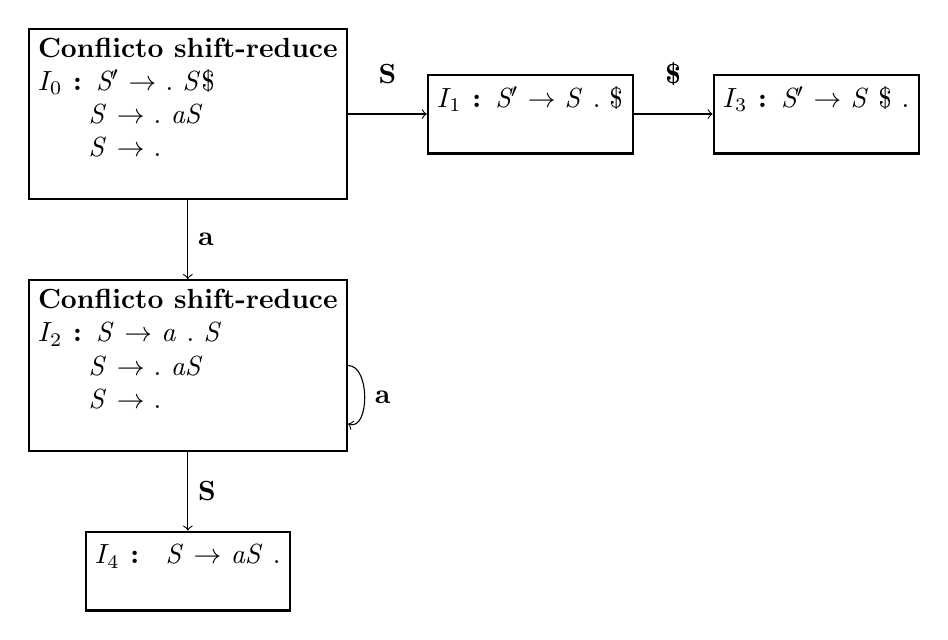
\begin{tikzpicture}[every node/.style={minimum height={1cm},thick,align=left}]
					
					\node[draw] (I0) {
						\textbf{Conflicto shift-reduce}\\
						\textbf{$I_0$ : }\textit{S$'$} $\rightarrow$ \textbf{$.$} \textit{S}\$\\
					   	$\hphantom{\quad}\hspace{5pt}$ \textit{S} $\rightarrow$ \textbf{$.$} \textit{aS}\\
						$\hphantom{\quad}\hspace{5pt}$ \textit{S} $\rightarrow$ \textbf{$.$}\\
					};
					\node[draw, right= of I0] (I1) {
						\textbf{$I_1$ : }\textit{S$'$} $\rightarrow$ \textit{S} \textbf{$.$} \$\\
					};
					\node[draw, below=of I0] (I2) {
						\textbf{Conflicto shift-reduce}\\
						\textbf{$I_2$ : }\textit{S} $\rightarrow$ \textit{a} \textbf{$.$} \textit{S}\\
						$\hphantom{\quad}\hspace{5pt}$ \textit{S} $\rightarrow$ \textbf{$.$} \textit{aS}\\
						$\hphantom{\quad}\hspace{5pt}$ \textit{S} $\rightarrow$ \textbf{$.$}\\
					};
					\node[draw, right=of I1] (I3) {
						\textbf{$I_3$ : }\textit{S$'$} $\rightarrow$ \textit{S} \$ \textbf{$.$}\\
					};
					\node[draw, below=of I2] (I4) {
						\textbf{$I_4$ : } \textit{S} $\rightarrow$ \textit{aS} \textbf{$.$}\\
					};

					\draw[->] (I0) -- (I1) node[midway,above] {\textbf{S}};
					\draw[->] (I0) -- (I2) node[midway,right] {\textbf{a}};
					\draw[->] (I1) -- (I3) node[midway,above] {\textbf{\$}};
					\draw[->] (I2) to [out=0,in=-20] node[midway,right] {\textbf{a}} (I2);
					\draw[->] (I2) -- (I4) node[midway,right] {\textbf{S}};
					\end{tikzpicture}

					
					Resolvemos el conflicto calculando el \textit{First} y después el \textit{Follow} y usamos este último para saber
					como resolver el \textbf{shift-reduce}:\\
		
					\begin{center}
						\begin{tabular}{| c | c | c |}
							\hline & \textbf{FIRST} & \textbf{FOLLOW} \\
							\hline \textbf{S'} & a,$\lambda$ & \$ \\
							\hline \textbf{S} & a,$\lambda$ & \$ \\
							\hline
						\end{tabular} \\
					\end{center}
	
					Luego, procedemos a crear la \textbf{Tabla de Parsing}, que queda:\\
					
					\begin{center}
						\begin{tabular}{| c | c | c | c | c |}
							\hline
							\textbf {Estado} & \multicolumn{2}{|c|}{\textbf{Acciones}} & \multicolumn{2}{|c|}{\textbf{Go to}} \\
							\hline & \textbf{a} & \textbf{\$} & \textbf{S'} & \textbf{S} \\
							\hline \textbf{$I_0$} & avanzar(2) & reducir(iii) & & 1 \\
							\hline \textbf{$I_1$} & & avanzar(3) & & \\
							\hline \textbf{$I_2$} & avanzar(2) & reducir(iii) &  & 4 \\
							\hline \textbf{$I_3$} &  & aceptar &  & \\
							\hline \textbf{$I_4$} & \multicolumn{2}{|c|}{reducir(ii)} &  & \\
							\hline
						\end{tabular}\\
					\end{center}
		
					Así, vemos que ésta gramática es finalmente \textit{LR(1)}.\\

				\item En términos de espacio, para la eficiencia de los analizadores de ambas gramáticas, tenemos que $G1_i$
					tiene sólo 4 estados en su tabla de parseo, mientras que $G1_d$ tiene 5 estados, así, la cantidad de pila y pasos utilizados para el reconocimiento de cualquier palabra perteneciente a \textit{L(a*)} es menor en $G1_i$ . En cuanto al 
					tiempo que le tomaría a cada autómata de pila en reconocer una frase de \textit{L(a*)} seguiría siendo menor para 
					el autómata de $G1_i$.\\

					Finalmente, la complejidad es \textbf{O(n)} para ambos puesto que en ambos casos la complejidad es lineal y depende
					del tamaño de la frase perteneciente al lenguaje.

			\end{enumerate}
		\item
		\begin{enumerate}[label=(\alph*)]
			\item Basados en la gramática dada, construimos un analizador sintáctico, empezando por transformar la gramática a:\\
			\begin{enumerate}[label=(\roman*)]
				\item \textit{Instr$'$} $\rightarrow$ \textit{Instr}\$\\
				\item \textit{Instr} $\rightarrow$ \textit{Instr$;$Instr}\\
				\item $\hphantom{\quad}\hspace{20pt}|$ \textit{IS}\\  
			\end{enumerate}

			Vemos que ocurre un conflicto \textbf{shift-reduce} en el estado $I_5$, como se ve en los siguientes estados:\\
							
			
			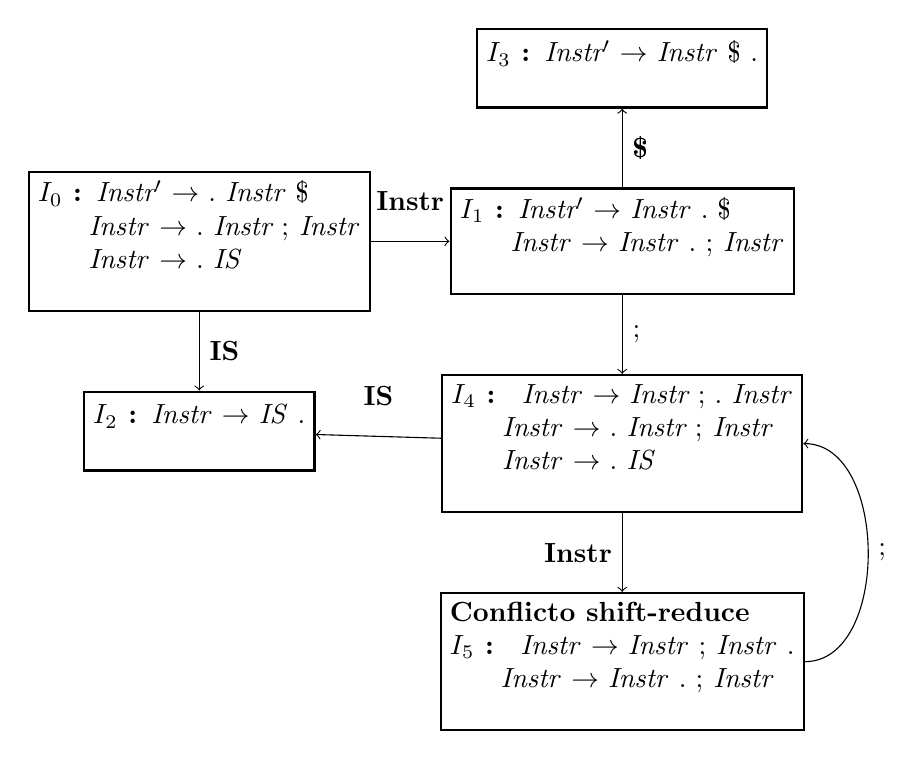
\begin{tikzpicture}[every node/.style={minimum height={1cm},thick,align=left}]
					
					\node[draw] (I0) {
						\textbf{$I_0$ : }\textit{Instr$'$} $\rightarrow$ \textbf{$.$} \textit{Instr} \$\\
					   	$\hphantom{\quad}\hspace{5pt}$ \textit{Instr} $\rightarrow$ \textbf{$.$} \textit{Instr $;$ Instr}\\
						$\hphantom{\quad}\hspace{5pt}$ \textit{Instr} $\rightarrow$ \textbf{$.$} \textit{IS}\\
					};
					\node[draw, right= of I0] (I1) {
						\textbf{$I_1$ : }\textit{Instr$'$} $\rightarrow$ \textit{Instr} \textbf{$.$}  \$\\
						$\hphantom{\quad}\hspace{5pt}$ \textit{Instr} $\rightarrow$ \textit{Instr} \textbf{$.$} \textit{$;$ Instr}\\
					};
					\node[draw, below=of I0] (I2) {
						\textbf{$I_2$ : }\textit{Instr} $\rightarrow$ \textit{IS} \textbf{$.$}\\
					};
					\node[draw, above=of I1] (I3) {
						\textbf{$I_3$ : }\textit{Instr$'$} $\rightarrow$ \textit{Instr} \$ \textbf{$.$}\\
					};
					\node[draw, below=of I1] (I4) {
						\textbf{$I_4$ : } \textit{Instr} $\rightarrow$ \textit{Instr $;$} \textbf{$.$} \textit{Instr}\\
					   	$\hphantom{\quad}\hspace{5pt}$ \textit{Instr} $\rightarrow$ \textbf{$.$} \textit{Instr $;$ Instr}\\
						$\hphantom{\quad}\hspace{5pt}$ \textit{Instr} $\rightarrow$ \textbf{$.$} \textit{IS}\\
					};
					\node[draw, below=of I4] (I5) {
						\textbf{Conflicto shift-reduce}\\
						\textbf{$I_5$ : } \textit{Instr} $\rightarrow$ \textit{Instr} \textit{$;$ Instr} \textbf{$.$}\\
					   	$\hphantom{\quad}\hspace{5pt}$ \textit{Instr} $\rightarrow$ \textit{Instr} \textbf{$.$} \textit{$;$ Instr}\\
					};


					\draw[->] (I0) -- (I1) node[midway,above] {\textbf{Instr}};
					\draw[->] (I0) -- (I2) node[midway,right] {\textbf{IS}};
					\draw[->] (I1) -- (I3) node[midway,right] {\textbf{\$}};
					\draw[->] (I1) -- (I4) node[midway,right] {\textbf{$;$}};
					\draw[->] (I4) -- (I2) node[midway,above] {\textbf{IS}};
					\draw[->] (I4) -- (I5) node[midway,left] {\textbf{Instr}};
					\draw[->] (I5) to [out=0,in=0] node[midway,right] {\textbf{$;$}} (I4);
					\end{tikzpicture}


			Tratamos de resolver el conflicto calculando el \textit{First} y después el \textit{Follow} y usamos este último para saber
			como resolver el \textbf{shift-reduce}:\\
		
			\begin{center}
				\begin{tabular}{| c | c | c |}
					\hline & \textbf{FIRST} & \textbf{FOLLOW} \\
					\hline \textbf{S'} & a, $\lambda$ & \$ \\
					\hline \textbf{S} & a, $\lambda$ & \$ \\
					\hline
				\end{tabular} \\
			\end{center}

			Luego vemos que en la \textbf{Tabla de Parsing} hay un conflicto pues con \textbf{$;$} puedo tanto avanzar como reducir al mismo tiempo y no hay forma de decidir exactamente cuál seguir siempre, luego, no es \textit{LR(1)}.\\

			\item Aún cuando existe un conflicto \textbf{shift-reduce} en el estado $I_5$ para el símbolo $;$ construiremos la \textbf{Tabla de Parsing} con conflictos, la cual quedaría de la siguiente forma:\\

			\begin{center}
				\begin{tabular}{| c | c | c | c | c | c |}
					\hline
					\textbf {Estado} & \multicolumn{3}{|c|}{\textbf{Acciones}} & \multicolumn{2}{|c|}{\textbf{Go to}} \\
					\hline & \textbf{$;$} & \textbf{IS} & \textbf{\$} & \textbf{Instr$'$} & \textbf{Instr} \\
					\hline \textbf{$I_0$} &  & avanzar(2) & & & 1 \\
					\hline \textbf{$I_1$} & avanzar(4) & & avanzar(3) & & \\
					\hline \textbf{$I_2$} & \multicolumn{3}{|c|}{reducir(iii)} & & \\
					\hline \textbf{$I_3$} & & & aceptar & & \\
					\hline \textbf{$I_4$} & & avanzar(2) & & & 5 \\
					\hline \textbf{$I_5$} & avanzar(4)$//$ reducir(ii) & & reducir(ii) & & \\
					\hline
				\end{tabular}\\
			\end{center}

			\item Para el reconocimiento de la frase \textit{IS;IS;IS} priorizaremos al shift y después al reduce:\\
			Priorizando el shift \textbf(avanzar):

			\begin{center}
				\begin{tabular}{| c | c | c |}
					\hline
					\textbf{Pila} & \textbf{Entrada} & \textbf{Acción}	\\
					\hline
					$I_0$ & IS;IS;IS\$ & avanzar(2) \\
					\hline
					$I_2$ $I_0$ & ;IS;IS\$ & reducir(iii)  \\
					\hline
					$I_1$ $I_0$ & ;IS;IS\$ & avanzar(4)  \\
					\hline
					$I_4$ $I_1$ $I_0$ & IS;IS\$ & avanzar(2) \\
					\hline
					$I_2$ $I_4$ $I_1$ $I_0$ & ;IS\$ & reducir(iii) \\
					\hline
					$I_5$ $I_4$ $I_1$ $I_0$ & ;IS\$ & avanzar(4)  \\
					\hline
				    $I_4$ $I_5$ $I_4$ $I_1$ $I_0$ & IS\$ & avanzar(2)  \\
					\hline
					$I_2$ $I_4$ $I_5$ $I_4$ $I_1$ $I_0$ & \$ & reducir(iii)  \\
					\hline
				    $I_5$ $I_4$ $I_5$ $I_4$ $I_1$ $I_0$ & \$ & reducir(ii)  \\
					\hline
					$I_5$ $I_4$ $I_1$ $I_0$ & \$ & reducir(ii)  \\
					\hline
				    $I_1$ $I_0$ & \$ & avanzar(3)  \\
					\hline
					$I_3$ $I_1$ $I_0$ & \$ & aceptar  \\
					\hline
				\end{tabular} \\
			\end{center}

			Priorizando el reduce \textbf(reducir):

			\begin{center}
				\begin{tabular}{| c | c | c |}
					\hline
					\textbf{Pila} & \textbf{Entrada} & \textbf{Acción}	\\
					\hline
					$I_0$ & IS;IS;IS\$ & avanzar(2) \\
					\hline
					$I_2$ $I_0$ & ;IS;IS\$ & reducir(iii)  \\
					\hline
					$I_1$ $I_0$ & ;IS;IS\$ & avanzar(4)  \\
					\hline
					$I_4$ $I_1$ $I_0$ & IS;IS\$ & avanzar(2) \\
					\hline
					$I_2$ $I_4$ $I_1$ $I_0$ & ;IS\$ & reducir(iii) \\
					\hline
					$I_5$ $I_4$ $I_1$ $I_0$ & ;IS\$ & reducir(ii)  \\
					\hline
					$I_1$ $I_0$ & ;IS\$ & avanzar(4) \\
					\hline
					$I_4$ $I_1$ $I_0$ & IS\$ & avanzar(2) \\
					\hline
					$I_2$ $I_4$ $I_1$ $I_0$ & \$ & reducir(iii) \\
					\hline
					$I_5$ $I_4$ $I_1$ $I_0$ & \$ & reducir(ii) \\
					\hline
					$I_1$ $I_0$ & \$ & avanzar(3) \\
					\hline
					$I_3$ $I_1$ $I_0$ & \$ & aceptar \\
					\hline
				\end{tabular} \\
			\end{center}

			Como vemos en el primer caso se asocia a la izquierda y en la segunda a la derecha pero en verdad vemos que es indiferente pues 
			existe una ambigüedad en el lenguaje al existir dos árboles sintácticos para la misma gramática.

			\item En cuanto al tamaño de la pila, el favorecer al \textbf{reduce} hace que la pila no sea tan grande y comparta la cantidad de pasos con el caso de favorecer al \textbf{shift}. En terminos de complejidad, para una frase IS;$(IS)^n$ vemos que conviene el uso de la segunda alternativa ya que se empilarían menos estados a la pila y por ende se harían menos operaciones de empilar y desempilar, lo que llevaría a una complejidad del tipo \textbf{O(n)} al depender de la cantidad de $';IS'$.

			\end{enumerate}
		\end{enumerate}
	\blfootnote{Benjamin Amos \#12-10240, Douglas Torres \#11-11027 / Enero - Marzo 2016}				 		
	
			
\end{document}
